\documentclass[../main.tex]{subfiles}

\graphicspath{{../images/}}

% sum commands

\begin{document}

\setcounter{section}{1}
\begin{center}
    \addcontentsline{toc}{section}{Homework 1}
    \section*{Homework 1}
    \subsection*{Due 1/30 12pm}
\end{center}
\hrule \vspace{10px}

\paragraph{1.}(a)
For case 1.1 the marginal probabilty is
\begin{align*}
    P(x = 0) = 0.2, \quad P(x = 1) = 0.8 \\
    P(y = 0) = 0.6, \quad P(y = 1) = 0.4
\end{align*}
For 1.2
\begin{align*}
    P(x = 0) = 0.4, \quad P(x = 1) = 0.6 \\
    P(y = 0) = 0.6, \quad P(y = 1) = 0.4
\end{align*}
(b) 1.1
\begin{align*}
    P(x=0 | y=0) = 1/5, \quad P(x=1 | y=0) = 4/5 \\
    P(x=0 | y=1) = 1/5, \quad P(x=1 | y=1) = 4/5
\end{align*}
1.2
\begin{align*}
    P(x=0 | y=0) = 1/3, \quad P(x=1 | y=0) = 2/3 \\
    P(x=0 | y=1) = 3/7, \quad P(x=1 | y=1) = 4/7
\end{align*}
(c) Variables $x$ and $y$ are independent iff $P(x,y) = P(x)P(y)$. For 1.1
\begin{gather*}
    P(x=0, y=0) = 0.12 \qand P(x=0) P(y=0) = 0.2(0.6) = 0.12 \\
    P(x=0, y=1) = P(x=0) P(y=1) = 0.2(0.4) = 0.08 \dots \\
    P(x,y) = P(x)P(y)
\end{gather*}
So $x$ and $y$ are independent for 1.1. You can also see that the condition of $y$ does not change
the marginal probability of $x$. For 1.2 there is a simple counterexample
\begin{gather*}
    P(x=0, y=0) = 0.1 \qand P(x=0) P(y=0) = 0.4(0.3) = 0.12 \\
    P(x=0, y=0) \neq P(x)P(y)
\end{gather*}
So $x$ and $y$ are not independent (dependent) for 1.2. You can also see that the conditional
probability is not the same as the marginal probability for both cases.

\paragraph{2.} For two random variables $x$ and $y$ to be independent, it must be true that
\begin{align} \label{eq:hw1} \tag{1}
    P(x,y) = P(x)P(y)
\end{align}
and from the definition of conditional probability
\begin{align*}
    P(x|y=y_o) &= \frac{P(x,y=y_o)}{P(y=y_o)}
\end{align*}
substituting \eqref{eq:hw1} into the joint probability
\begin{align*}
    P(x|y=y_o) &= \frac{P(x)P(y=y_o)}{P(y=y_o)} \\
    P(x|y=y_o) &= P(x)
\end{align*}

\paragraph{3.}(a) Since the two thrown dice are independent, the fair dice has 36 possible outcomes
$A_{xy} = \{ (1,1), (1,2), \dots, (6,6) \}$ with equal probability
\begin{align*}
    P(x,y) = P(x)P(y) = \frac{1}{6} \cdot \frac{1}{6} = \frac{1}{36}
\end{align*}
The probability distribution of the sum of the two dice $P(S)$ is
\begin{align*}
    P(S) = \begin{cases}
        1/36 & S = 2, 12 \\
        2/36 & S = 3, 11 \\
        3/36 & S = 4, 10 \\
        4/36 & S = 5, 9 \\
        5/36 & S = 6, 8 \\
        6/36 & S = 7
    \end{cases}
\end{align*}
where $S = x + y$. For the absolute difference of the two dice $D = |x - y|$
\begin{align*}
    P(D) = \begin{cases}
        2/36 & D = 5 \\
        4/36 & D = 4 \\
        6/36 & D = 3 \\
        8/36 & D = 2 \\
        10/36 & D = 1 \\
        6/36 & D = 0
    \end{cases}
\end{align*}
for the difference $D = 0$ there are 6 possible outcomes $(1,1), (2,2), \dots, (6,6)$, for $D = 1$
there are 10 possible outcomes $(1,2), (2,1), (2,3), (3,2), \dots, (5,6), (6,5)$, and so on. 

(b) For 100 dice, the probability distribution of the sum of the dice $P(S)$ would be roughly
\begin{align*}
    P(S) = \begin{cases}
        1/6^{100} & S = 100, 600 \\
        100/6^{100} & S = 101, 599 \\
        5050/6^{100} & S = 102, 598 \\
        \vdots & \vdots \\
        \num{1.52e76}/6^{100} & S = 350 \\
    \end{cases}
\end{align*}
first we find the mean of 1 independent dice roll $(\mu_1)$':
\begin{align*}
    \mu_1 = \sum_{x} P(x) x = \frac{1}{6} \sum_{x=1}^{6} x = \frac{21}{6} = 3.5
\end{align*}
because the mean of $N$ independent dice rolls is the sum of the means of each dice roll
\begin{align*}
    \mu_N = \sum_{i=1}^{N} \mu_i
\end{align*}
thus the mean of 100 dice rolls is
\begin{align*}
    \mu_{100} = 100 \cdot \mu_1 = \boxed{350}
\end{align*}
To find the Standard Deviation we first find the variance of 1 independent dice roll $(\sigma_1^2)$:
\begin{align*}
    \Var[x] = \E[(x - \E[x])^2] &= \E[ x^2 - 2x\E[x] + \E[x]^2 ] \\
    &= \E[x^2] - 2\E[x]^2 + \E[x]^2\E[1] = \E[x^2] - \E[x]^2
\end{align*}
or in summation notation
\begin{align*}
    \sigma_1^2 = \sum_{x} P(x) (x - \mu_1)^2 = \frac{1}{6} \sum_{x=1}^{6} (x - 3.5)^2
    = \frac{17.5}{6} = 2.9167
\end{align*}
for 2 independent variables $x$ and $y$
\begin{align*}
    \Var[x + y] &= \E[((x + y) - \E[x + y])^2] \\
    &= \E[(x - \E[x]) + (y - \E[y])^2] \\
    &= \E[(x - \E[x])^2 + (y - \E[y])^2 + 2(x - \E[x])(y - \E[y])] \\
    &= \E[(x - \E[x])^2] + \E[(y - \E[y])^2] + 2\E[(x - \E[x])(y - \E[y])] \\
    &= \Var[x] + \Var[y] + 2\E[(x - \E[x])(y - \E[y])]
\end{align*}
where the third term is
\begin{align*}
    \E[(x - \E[x])(y - \E[y])] &= \E[xy - x\E[y] - y\E[x] + \E[x]\E[y]] \\
    &= \E[xy] - \E[x]\E[y]
\end{align*}
and for independent variables $x$ and $y$ the third term is zero. Thus the variance of the sum of
$N$ independent dice rolls is
\begin{align*}
    \Var[N] = N\sigma_1^2 = 100 \cdot 2.9167 = 291.67
\end{align*}
and the standard deviation is
\begin{align*}
    \sigma_N = \sqrt{\Var[N]} = \sqrt{291.67} = \boxed{17.08}
\end{align*}

% insert figure hw1_3b.png here
% change section counter to 3
\begin{figure}[ht]
    \centering
    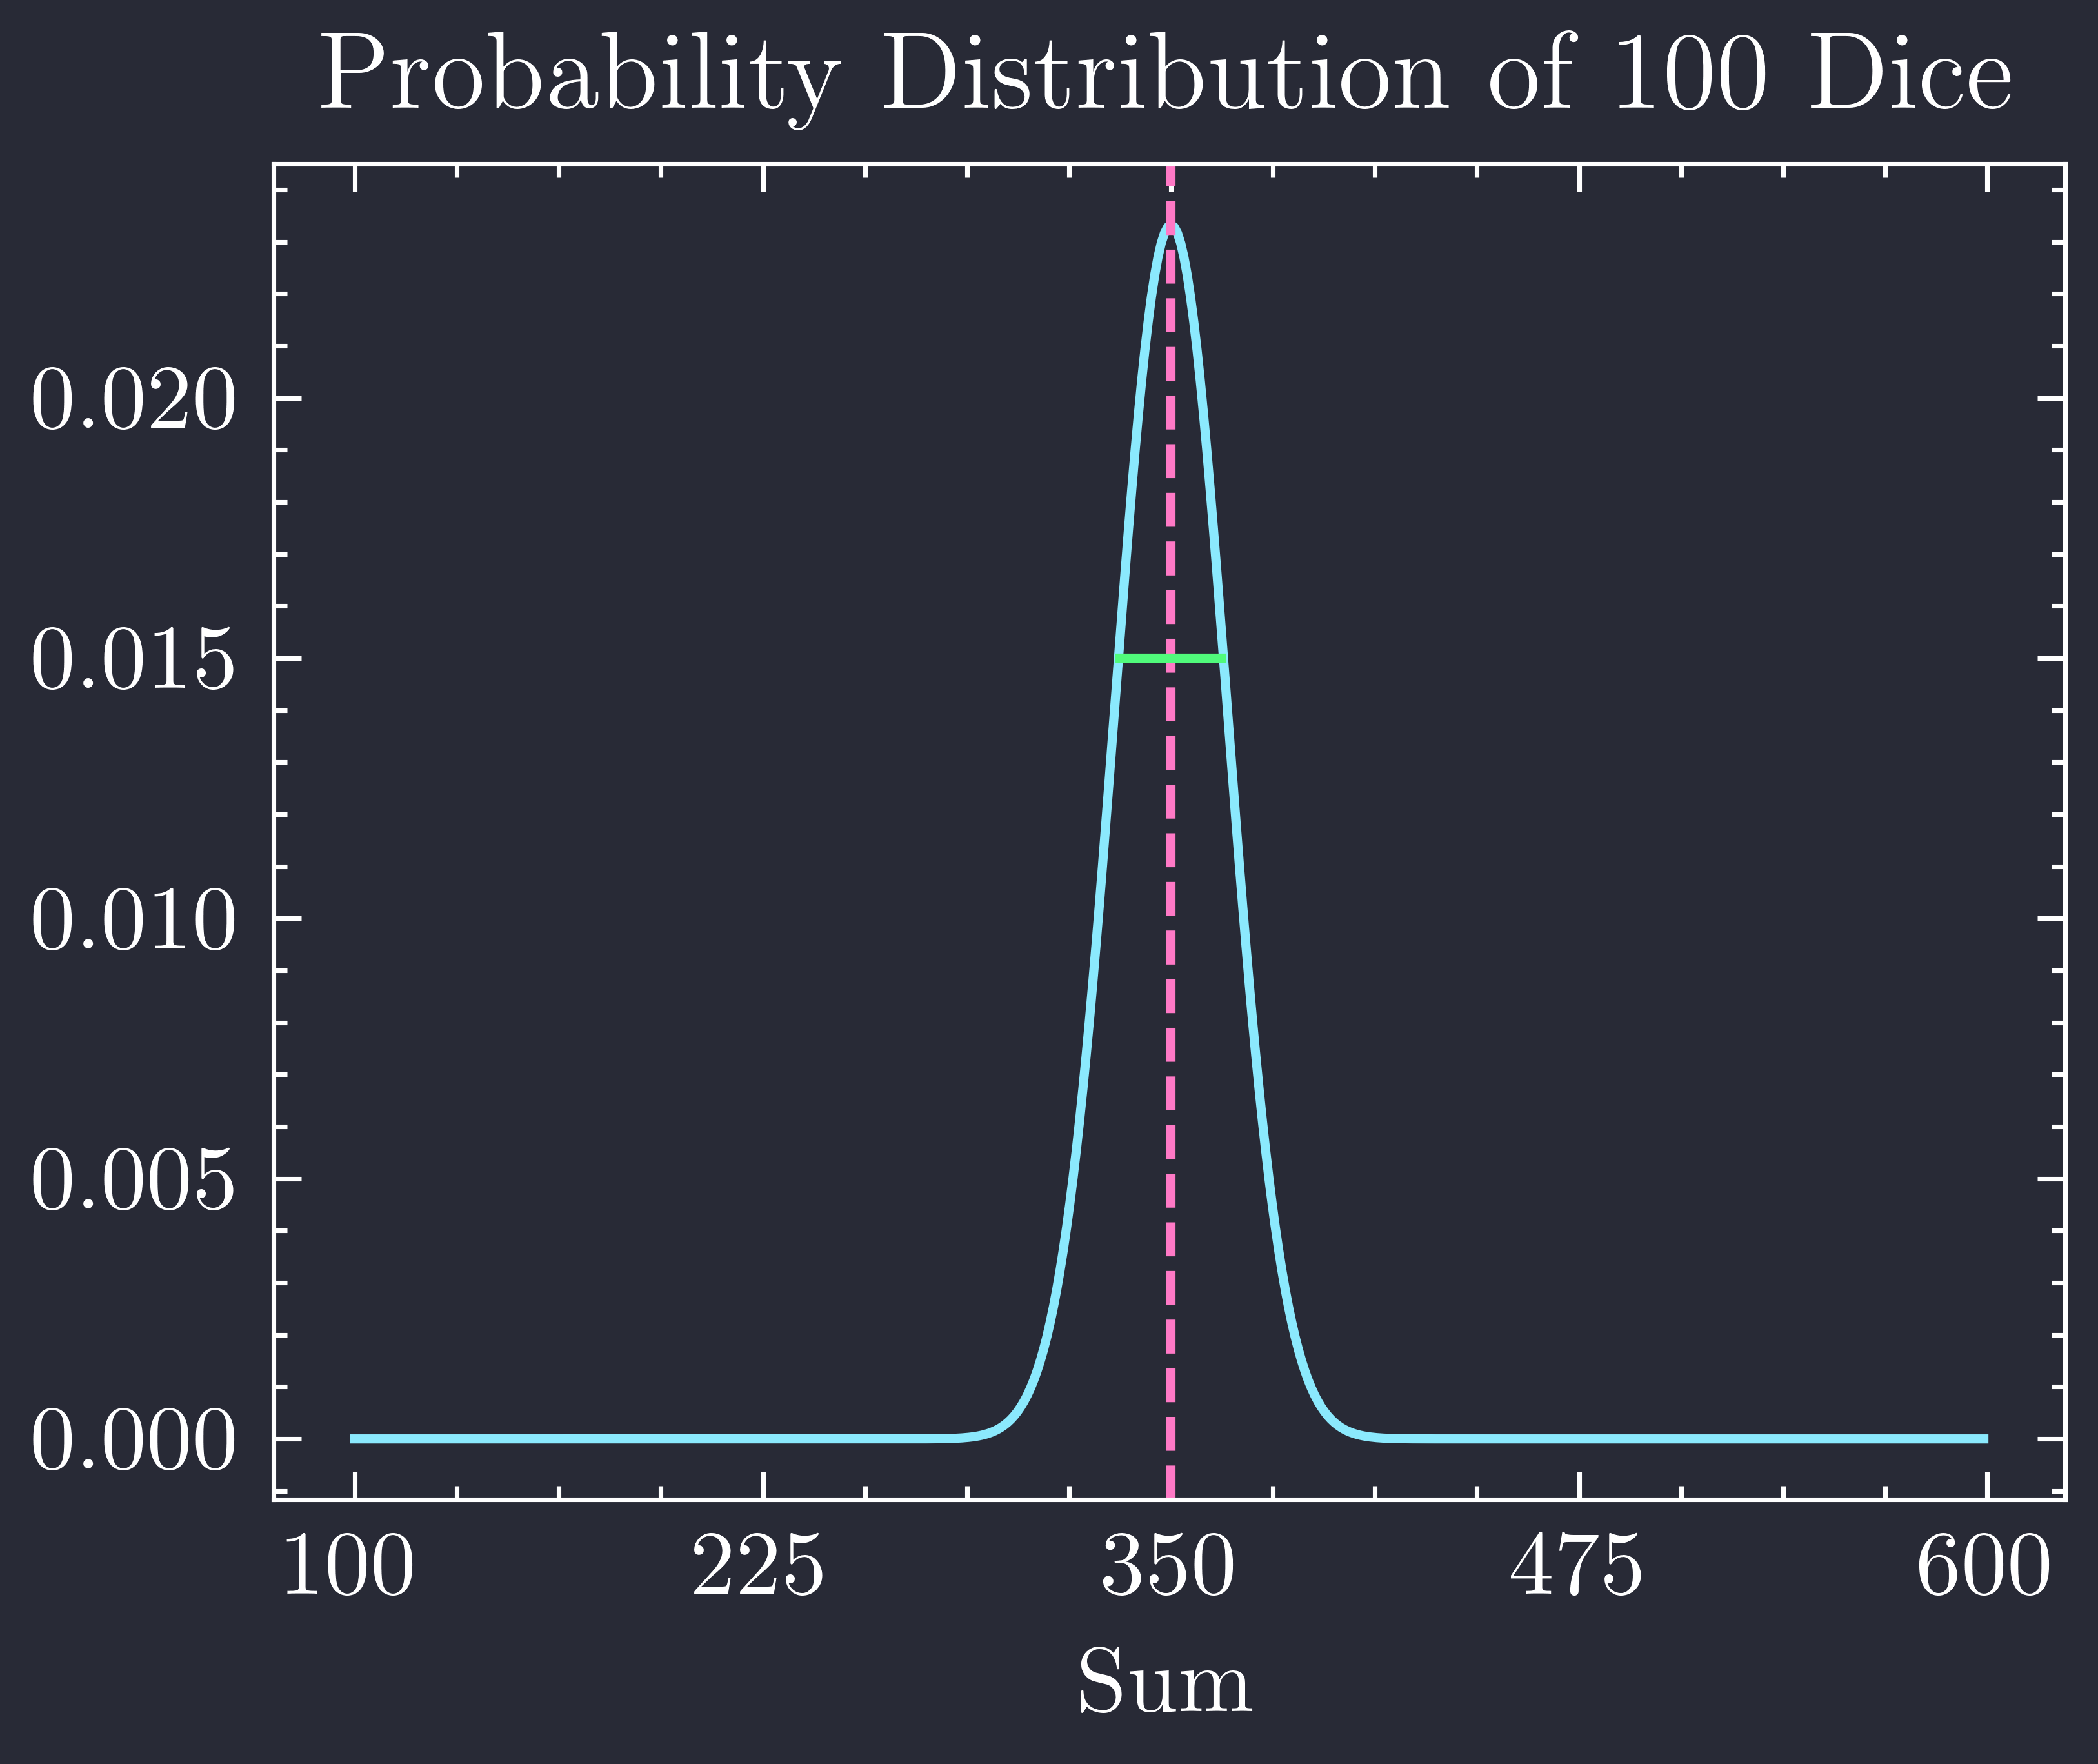
\includegraphics[width=0.5\linewidth]{hw1_3b.png}
    \captionsetup{width=0.8\linewidth}
    \caption{Probability distribution of the sum of 100 dice rolls. The mean is 350 and the
    standard deviation is $\approx 17$.}
    \label{fig:hw1_3b}
\end{figure}
The sketch of probability distribution of the sum of 100 dice rolls is shown in
Figure \ref{fig:hw1_3b}. 

\paragraph{4.} (a) Assuming that there is an equal likelihood of the order of the age of the three
brothers being any of the 6 possible permutations:
\begin{align*}
    \textrm{Age}_{A,B,F} = \qt{ABF, AFB, BAF, BFA, FAB, FBA}
\end{align*}
where we denote the first element of a permutation as the oldest brother and the last element as
the youngest brother.

The probability that Fred (F) is older than Bob 
(B) is $\boxed{1/2}$ from both the 3 possible permutations or by realizing that there are only two
equal outcomes when looking at only the age of Fred vs Bob.

(b) Given that Fred is older than Alex (A), we can eliminate the 3 permutations where Alex is older.
Thus the probability that Fred is older than Bob is $\boxed{2/3}$.

\paragraph{5.} (a) Given that the probability of choosing a black ball from an urn is
$f_B = \frac{B}{K}$, the probability distribution of choosing $n_B$ black balls from $N$ draws is
\begin{align*}
    \boxed{P(n_B | N, f_B) = \binom{N}{n_B} f_B^{n_B} (1 - f_B)^{N - n_B}}
\end{align*}
(b) Finding the mean and standard deviation of $n_B$ is quite similar to Problem 3. Since each draw
is independent, the mean of $n_B$ is the sum of the means of each draw! In the case of drawing one
ball has a binary outcome
\begin{align*}
    n_B(N = 1) = \begin{cases}
        1 & \textrm{black ball with probability } f_b \\
        0 & \textrm{white ball } (1 - f_B)
    \end{cases}
\end{align*}
thus the mean of $n_B$ for one draw is
\begin{align*}
    \mu_1 = 1 (f_B) + 0 (1 - f_B) = f_B
\end{align*}
and the variance is 
\begin{align*}
    \sigma_1^2 = (1 - f_B)^2 f_B + (0 - f_B)^2 (1 - f_B) = f_B(1 - f_B)
\end{align*}
for $N$ draws the means add up to
\begin{align*}
    \boxed{\mu = N f_B}
\end{align*}
and the variances add only due to the independent nature of the draws
\begin{align*}
    \sigma^2 = N f_B (1 - f_B)
\end{align*}
thus the standard deviation is
\begin{align*}
    \boxed{\sigma = \sqrt{N f_B (1 - f_B)}}
\end{align*}
For $K = 20$, and $B = K$; $f_B = 5/20 = 0.25$. And for $N = 5$ we have the ratio
\begin{align*}
    \frac{\sigma}{\mu} = \frac{\sqrt{5 \cdot 0.25 \cdot 0.75}}{5 \cdot 0.25}
    = \frac{\sqrt{15}}{5} \approx \boxed{0.77}
\end{align*}
and for $N = 20$
\begin{align*}
    \frac{\sigma}{\mu} = \frac{\sqrt{1000 \cdot 0.25 \cdot 0.75}}{1000 \cdot 0.25} 
    = \frac{\sqrt{30}}{100} \approx \boxed{0.05}
\end{align*}

% do 6 possibly
\paragraph{6.} (a) Dividing the time period $T$ in to $M$ intervals where each interval has a 
probability $r \dd{t}$ or $\dd{t} = T/M$. The probability of no events occuring in time $T$ is
\begin{align*}
    \lim_{M \to \infty} \qt(1 - r \dd{t})^M = \lim_{M \to \infty} \qt(1 - \frac{rT}{M})^M =
    \boxed{ e^{-rT}}
\end{align*} 
(b) For $n_T = x$ events occuring in $M$ this is similar to the binomial distribution as $M \to \infty$. 
\begin{align*}
    \lim_{M \to \infty }\frac{M!}{x! (M - x)!} \qt(\frac{rT}{M})^x
        \qt(1 - \frac{rT}{M})^{M - x}
\end{align*}
canceling out some terms\dots
\begin{align*}
    \frac{M!}{(M-x)!} = \frac{M(M-1)\cdots(M-x+1)(M-x)!}{(M-x)!} = M(M-1)\cdots(M-x+1)
\end{align*}
and now the facorial has $x$ terms, so we can write it as
\begin{align*}
    \frac{M(M-1)\cdots(M-x+1)}{M^x} &= \frac{M}{M} \frac{M-1}{M} \cdots \frac{M-x+1}{M} \\
    &= 1 \cdot \qt(1 - \frac{1}{M}) \cdots \qt(1 - \frac{x-1}{M})
\end{align*}
and as $M \to \infty$ the terms in the product go to 1, so the product goes to 1. Thus we are left
with
\begin{align*}
    \lim_{M \to \infty } \frac{(rT)^x}{x!} \qt(1 - \frac{rT}{M})^{M - x} &=
    \lim_{M \to \infty } \frac{(rT)^x}{x!} \qt(1 - \frac{rT}{M})^{M}
    \qt(1 - \frac{rT}{M})^{-x}
\end{align*}
the second term is the limit of the exponential function
\begin{align*}
    \lim_{M \to \infty } \qt(1 - \frac{rT}{M})^{M} = e^{-rT}
\end{align*}
and the third term tends to 1 as $M \to \infty$. Thus the probability of $x$ events occuring in
time $T$ is
\begin{align*}
    \boxed{P(x) = \frac{(rT)^x}{x!} e^{-rT}}
\end{align*}
where $x = n_T$ for the sake of brevity in notation.

(c) The mean of $n_T$ is
\begin{align*}
    \mu &= \sum_{x=0}^{\infty} x P(x) \\
    &= \sum_{x=0}^{\infty} x \frac{(rT)^x}{x!} e^{-rT} \\
    &= e^{-rT} \sum_{x=1}^{\infty} x\frac{(rT)(rT)^{x-1}}{x(x-1)!} \\
    &= e^{-rT} (rT) \sum_{x=1}^{\infty} \frac{(rT)^{x-1}}{(x-1)!}
\end{align*}
the the first term of the sum is zero which is why the sum starts at $x = 1$. The sum is also
the Taylor series expansion of $e^{rT}$ if we let $n = x - 1$ so
\begin{align*}
    \sum_{x=1} \frac{(rT)^{x-1}}{(x-1)!} = \sum_{n=0} \frac{(rT)^n}{n!} = e^{rT}
\end{align*}
Therefore the mean of $n_T$ is
\begin{align*}
    \mu = (rT) e^{-rT} e^{rT} = rT
\end{align*}
The variance of $n_T$ is
\begin{align*}
    \sigma^2 &= \E[x^2] - \E[x]^2
\end{align*}
the first term is solved similarly to the mean
\begin{align*}
    \E[x^2] &= \sum_{x=0}^{\infty} x^2 P(x) \\
    &= \sum_{x=0}^{\infty} x^2 \frac{(rT)^x}{x!} e^{-rT} \\
    &= e^{-rT} \sum_{x=1}^{\infty} x^2 \frac{(rT)(rT)^{x-1}}{x(x-1)!} \\
    &= (rT) e^{-rT} \sum_{x=1}^{\infty} x \frac{(rT)^{x-1}}{(x-1)!} \\
    &= (rT) e^{-rT} \qt[\sum_{x=1}^{\infty} (x-1) \frac{(rT)^{x-1}}{(x-1)!} + 
    \sum_{x=1}^{\infty} \frac{(rT)^{x-1}}{(x-1)!}
    ] \qquad x = [(x - 1) + 1]\\
    &= (rT) e^{-rT} \qt[(rT)\sum_{x=2}^{\infty}  \frac{(rT)^{x-2}}{(x-2)!} +
    \sum_{n=0}^{\infty} \frac{(rT)^{n}}{n!}
    ] \qquad n = x - 1 \\
    &= (rT) e^{-rT} \qt[(rT)\sum_{l=0}^{\infty}  \frac{(rT)^{l}}{l!} +
    \sum_{n=0}^{\infty} \frac{(rT)^{n}}{n!}
    ] \qquad l = x - 2 \\
    &= (rT) e^{-rT} \qt[(rT) e^{rT} + e^{rT} ]  \\
    &= (rT)^2 e^{-rT} e^{rT} + (rT) e^{-rT} e^{rT} \\
    &= (rT)^2 + rT
\end{align*}
and the variance is
\begin{align*}
    \sigma^2 = (rT)^2 + rT - (rT)^2 = rT
\end{align*}
Therefore the mean and standard deviation of $n_T$ are
\begin{align*}
    \boxed{\mu = rT \qand \sigma = \sqrt{rT}}
\end{align*}
\paragraph{7.}
Using Bayes' theorem for the outcome $X = \qt{7,3,4,2,5,3}$ is 
\begin{align*}
    P(A | 7,3,4,2,5,3) = P(A | X)  = \frac{P( X | A) P(A)}{P(X)}
\end{align*}
where the probability of choosing dice A is 1 in 3---$P(A) = 1/3$. The conditional probabilty 
$P(X | A)$ is the probability of rolling the outcome $X$ given that dice A is chosen:
\begin{align*}
    P(X | A) = \frac{1 \times 4 \times 2 \times 4 \times 2 \times 4}{20^6} = \frac{256}{20^6}
\end{align*}
and the probability of rolling the outcome $X$ is given by the sum rule
\begin{align*}
    P(X) = P(X | A) P(A) + P(X | B) P(B) + P(X | C) P(C)
\end{align*}
where $P(B) = P(C) = 1/3$ and the conditional probabilities $P(X | B)$ and $P(X | C)$ are
\begin{align*}
    P(X | B) = \frac{2 \times 3 \times 2 \times 2 \times 2 \times 3}{20^6} = \frac{144}{20^6} \\
    P(X | C) = \frac{2^6}{20^6} = \frac{64}{20^6}
\end{align*}
thus the probability of choosing dice A given the outcome $X$ is
\begin{align*}
    P(A | X) = \frac{\frac{256}{20^6} \cdot \frac{1}{3}}{\frac{256}{20^6} \cdot \frac{1}{3} +
    \frac{144}{20^6} \cdot \frac{1}{3} + \frac{64}{20^6} \cdot \frac{1}{3}} = \frac{256}{464}
    \approx \boxed{0.55}
\end{align*}
with the knowledge that terms cancel out, the probability of the die being B is
\begin{align*}
    P(B | X) = \frac{144}{464} \approx \boxed{0.31}
\end{align*}
and the probability of the die being C is
\begin{align*}
    P(C | X) = \frac{64}{464} \approx \boxed{0.14}
\end{align*}

\paragraph{8.} (a) Given that the bus arrives on average every 5 minutes, the average wait time is
5 minutes. And the bus that just left Sally would have left an average of 5 minutes ago. From the
code, taking the mean value of the wait times is also $\approx 5$ minutes.

(b) Therefore the average time between two buses is the sum in the time Sally is waiting for
the bus and how long the missed bus has been gone: 10 minutes. 

(c) The paradox is that `we' think that after waiting for 5 minutes the bus will arrive, but the 
average time between buses is 10 minutes, so we are waiting longer than we expect to intuitively.
This is because the conditional probability of Sally getting to the bus stop where the interval 
between buses is less than 5 minutes given that she has waited for a time $t$ is less as time goes
on. And the probability that Sally arrived at the bus stop where the interval between buses is more
than 5 minutes given that she has waited for a time $t$ is more as time goes on.

(d)
\begin{figure} [h]
    \centering
    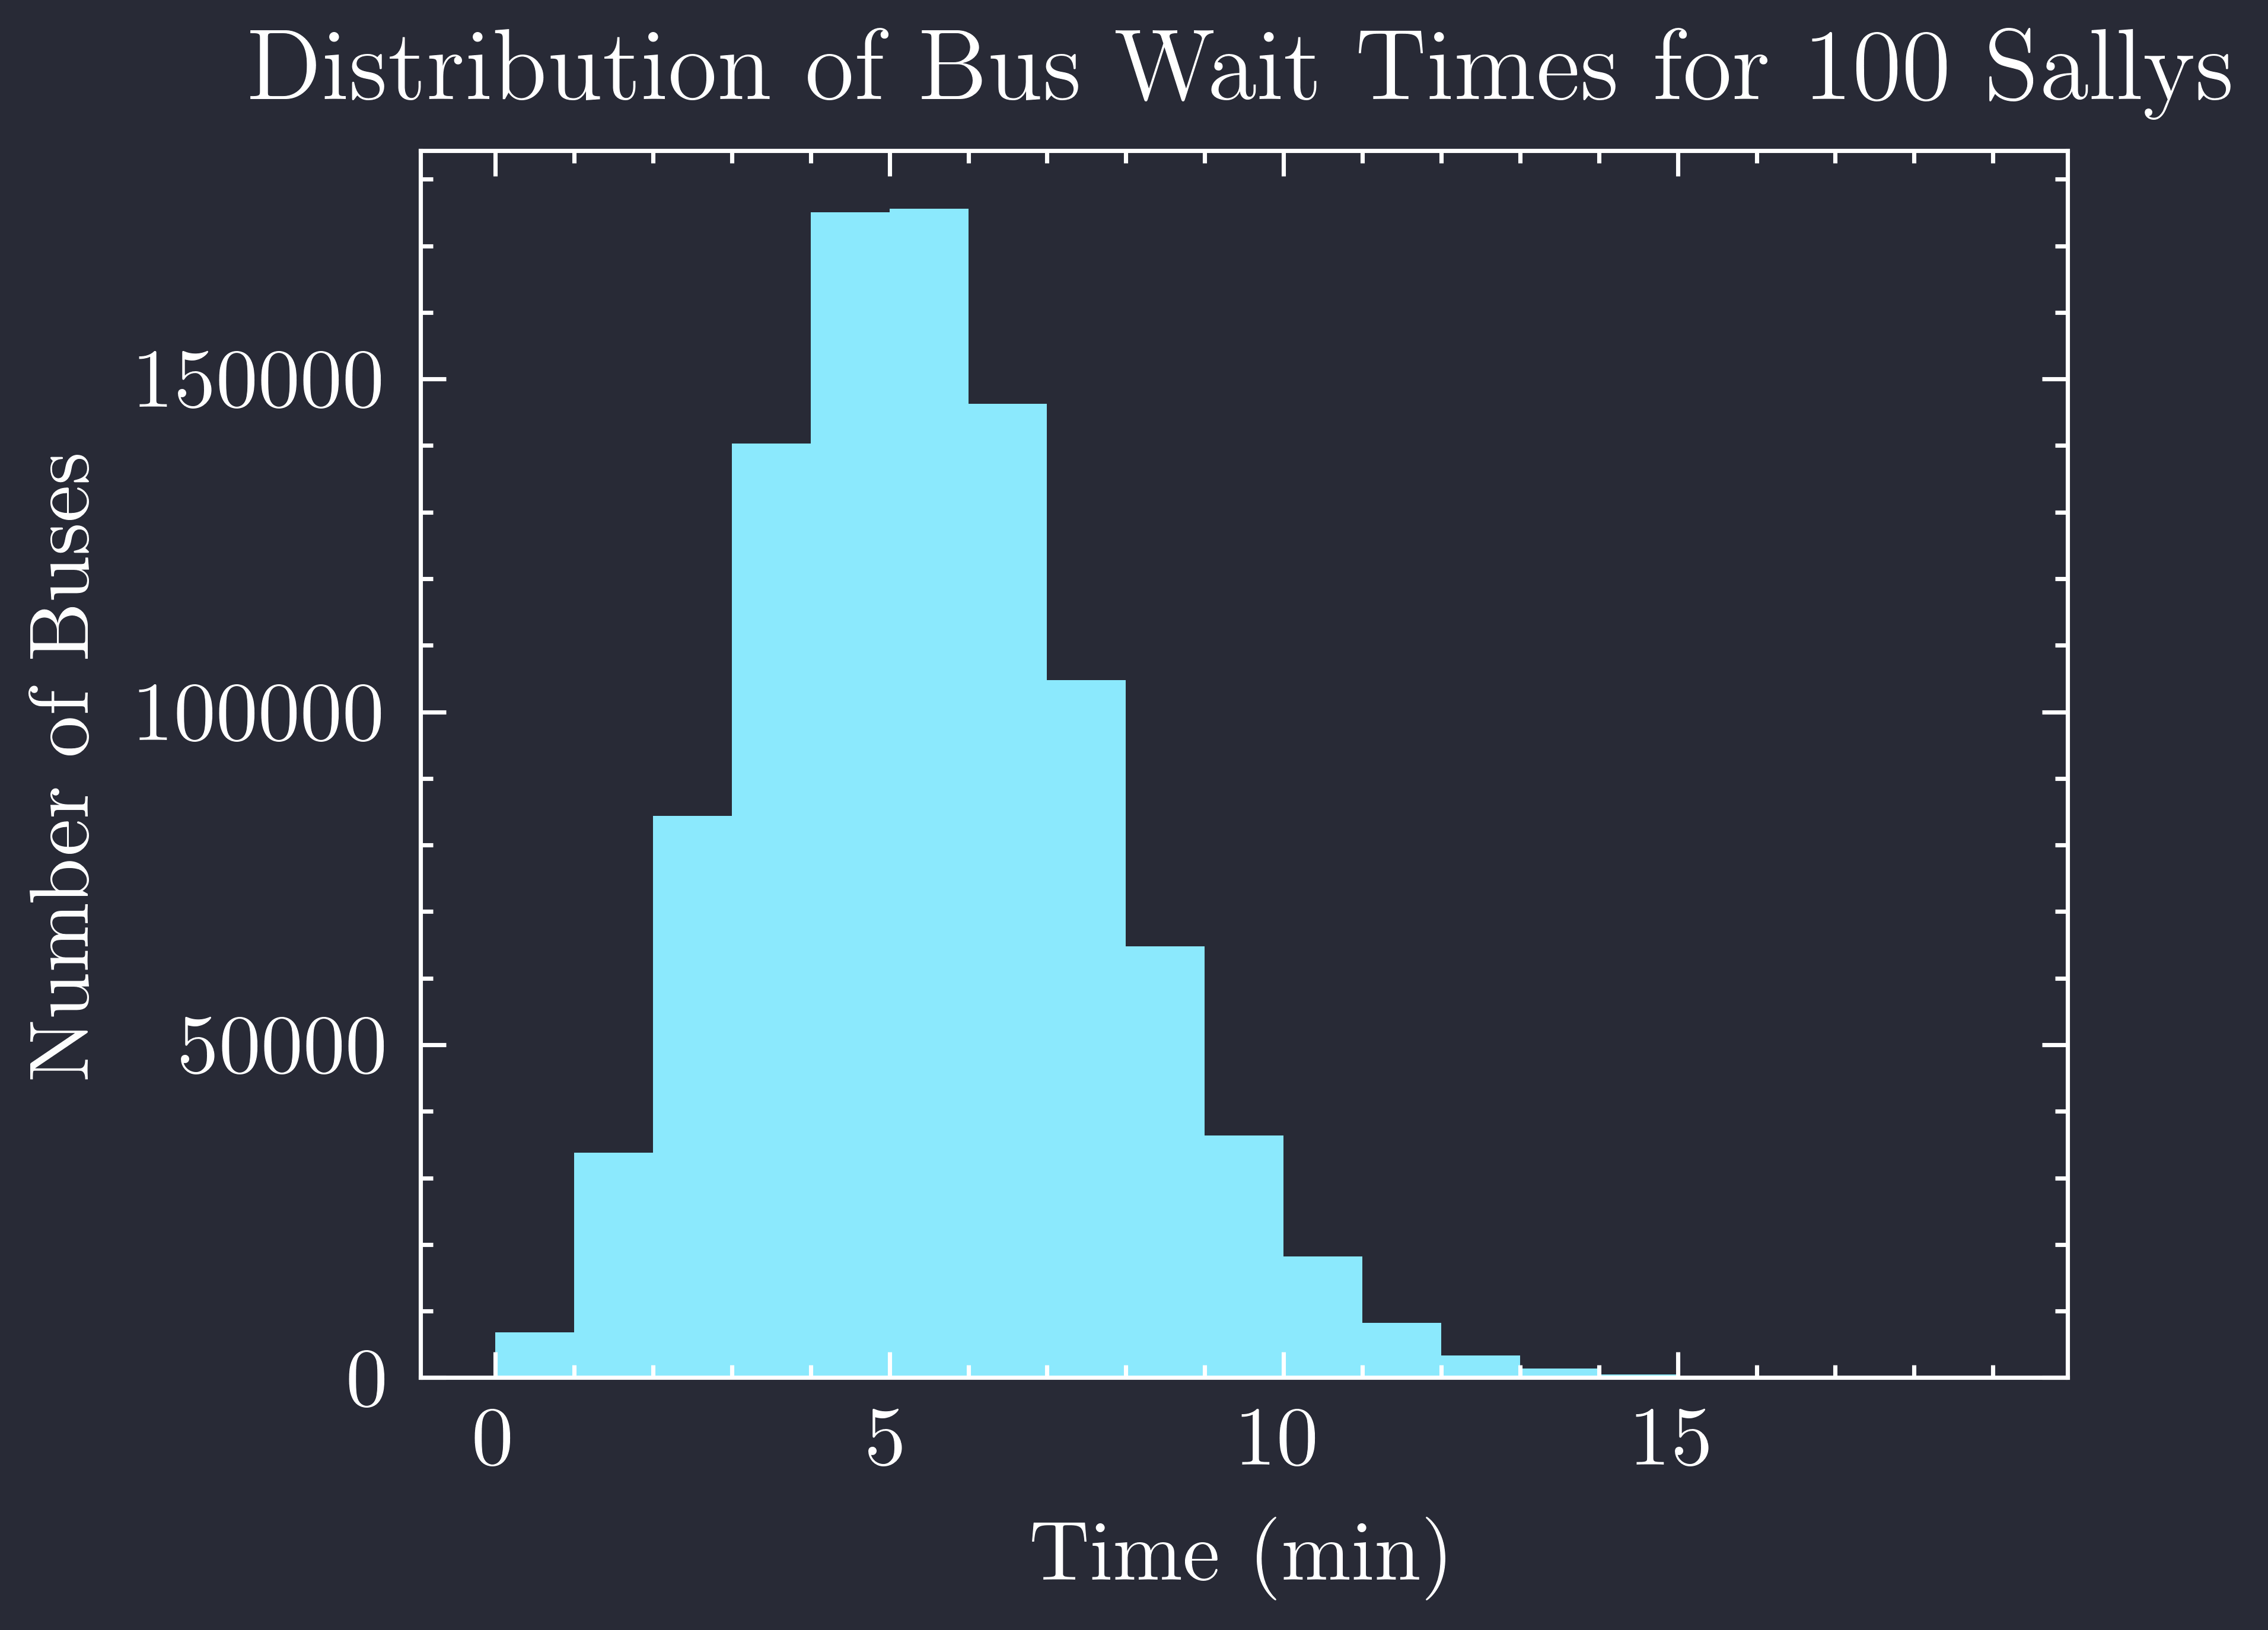
\includegraphics[width=0.7\linewidth]{hw1_8d.png}
    \caption{Mean of 5.00 min and Time between buses of 10.00 min.}
    \label{fig:hw1_8d}
\end{figure}

PYTHON CODE BELOW
% hw1_python.pdf
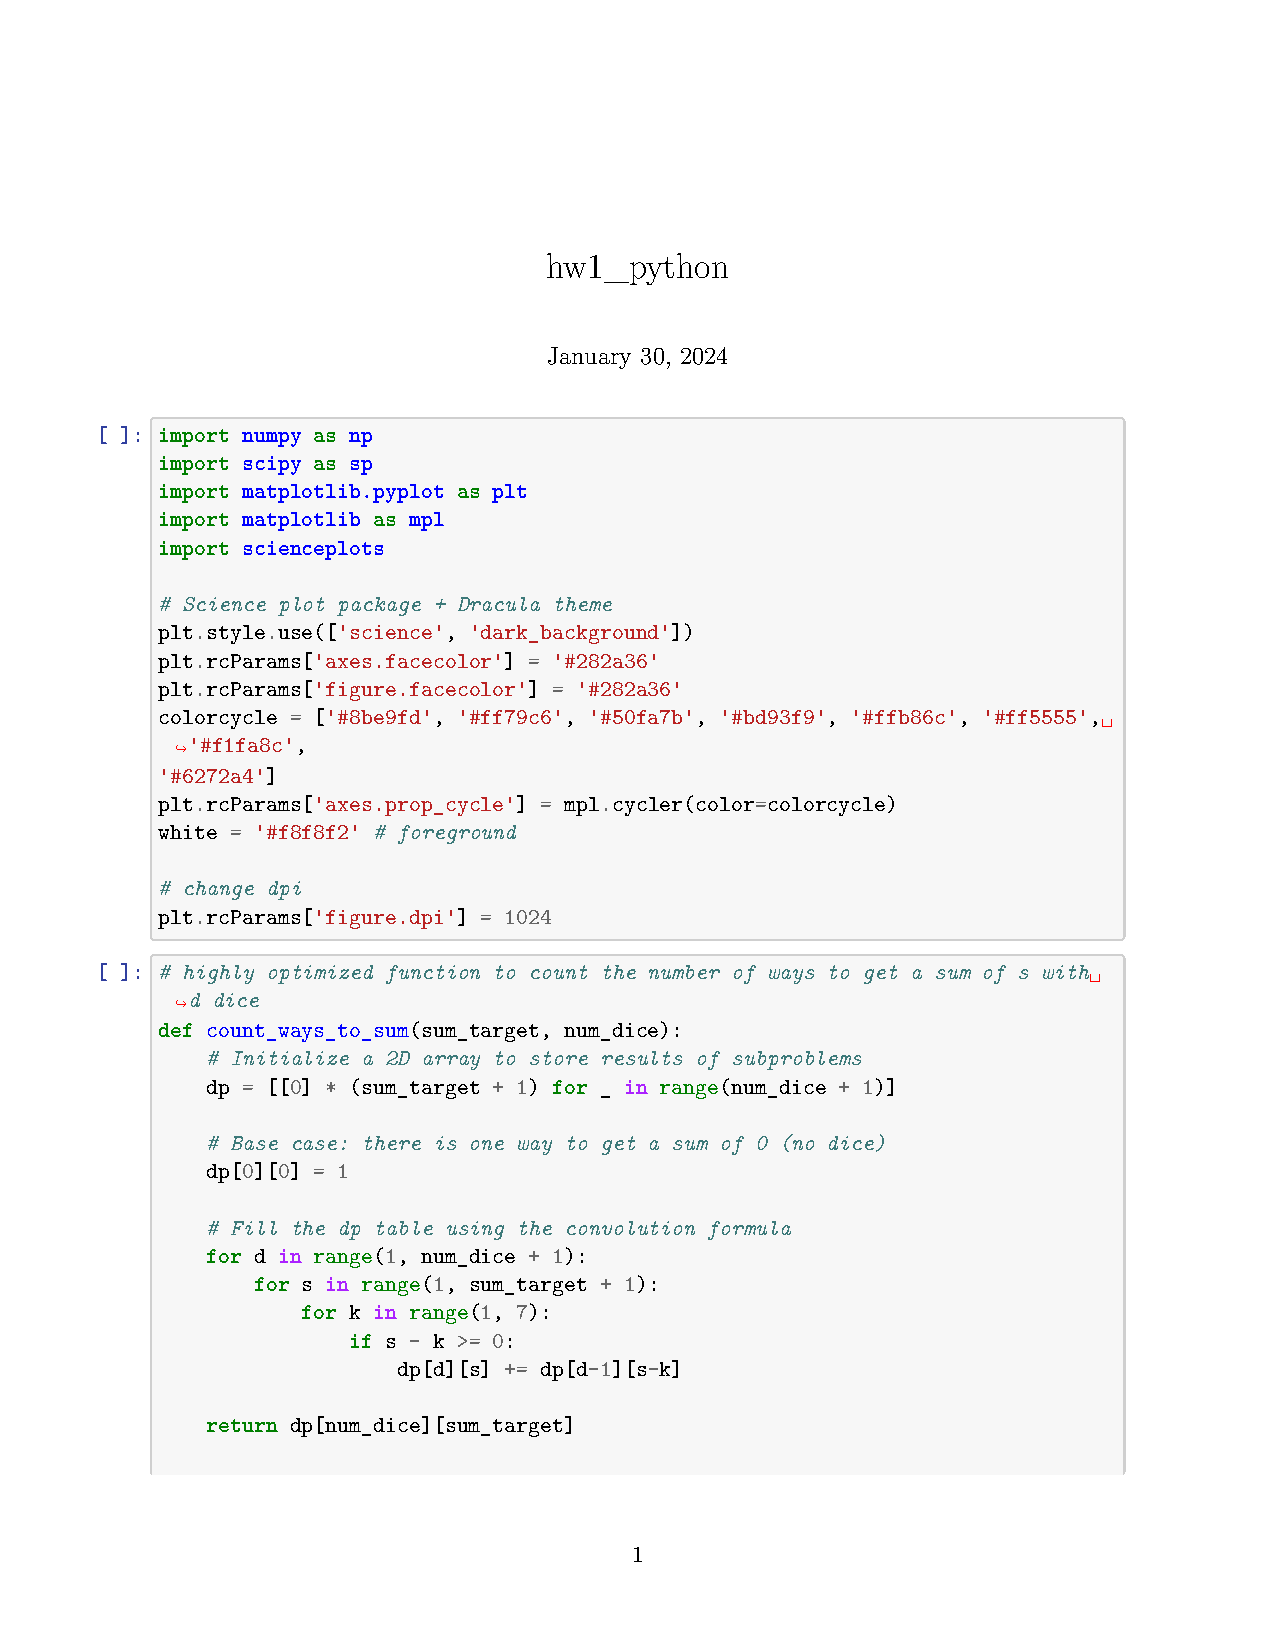
\includepdf[pages=-]{hw1_python.pdf}

\end{document}